\chapter{Synchronization System Case Study}
\etocsettocstyle{\rule{\textwidth}{1pt}}{\rule{\textwidth}{1pt}} % style for toc
\localtableofcontents
\label{chap:synchronization}

In eCommerce, synchronization systems are often needed to ensure that the online store reflects the current state of the store's products' logistics. Brick-and-mortar stores manage their inventory with logistical software system. A synchronization system that ensures the consistency and truthfulness of the online store is crucial.
The main focus of this chapter is on a practical comparison between serverless and monolithic implementations of such a synchronization system. Synthetic workloads are generated and two mock servers, simulating a logistics system and a Shopify store are used.
\section{Introduction}
Suppose a brick-and-mortar store sells products, for example shoes. A shoe may have different variants: shoes of the same model could come in different colors and sizes.
\begin{figure}[h!]
    \centering
    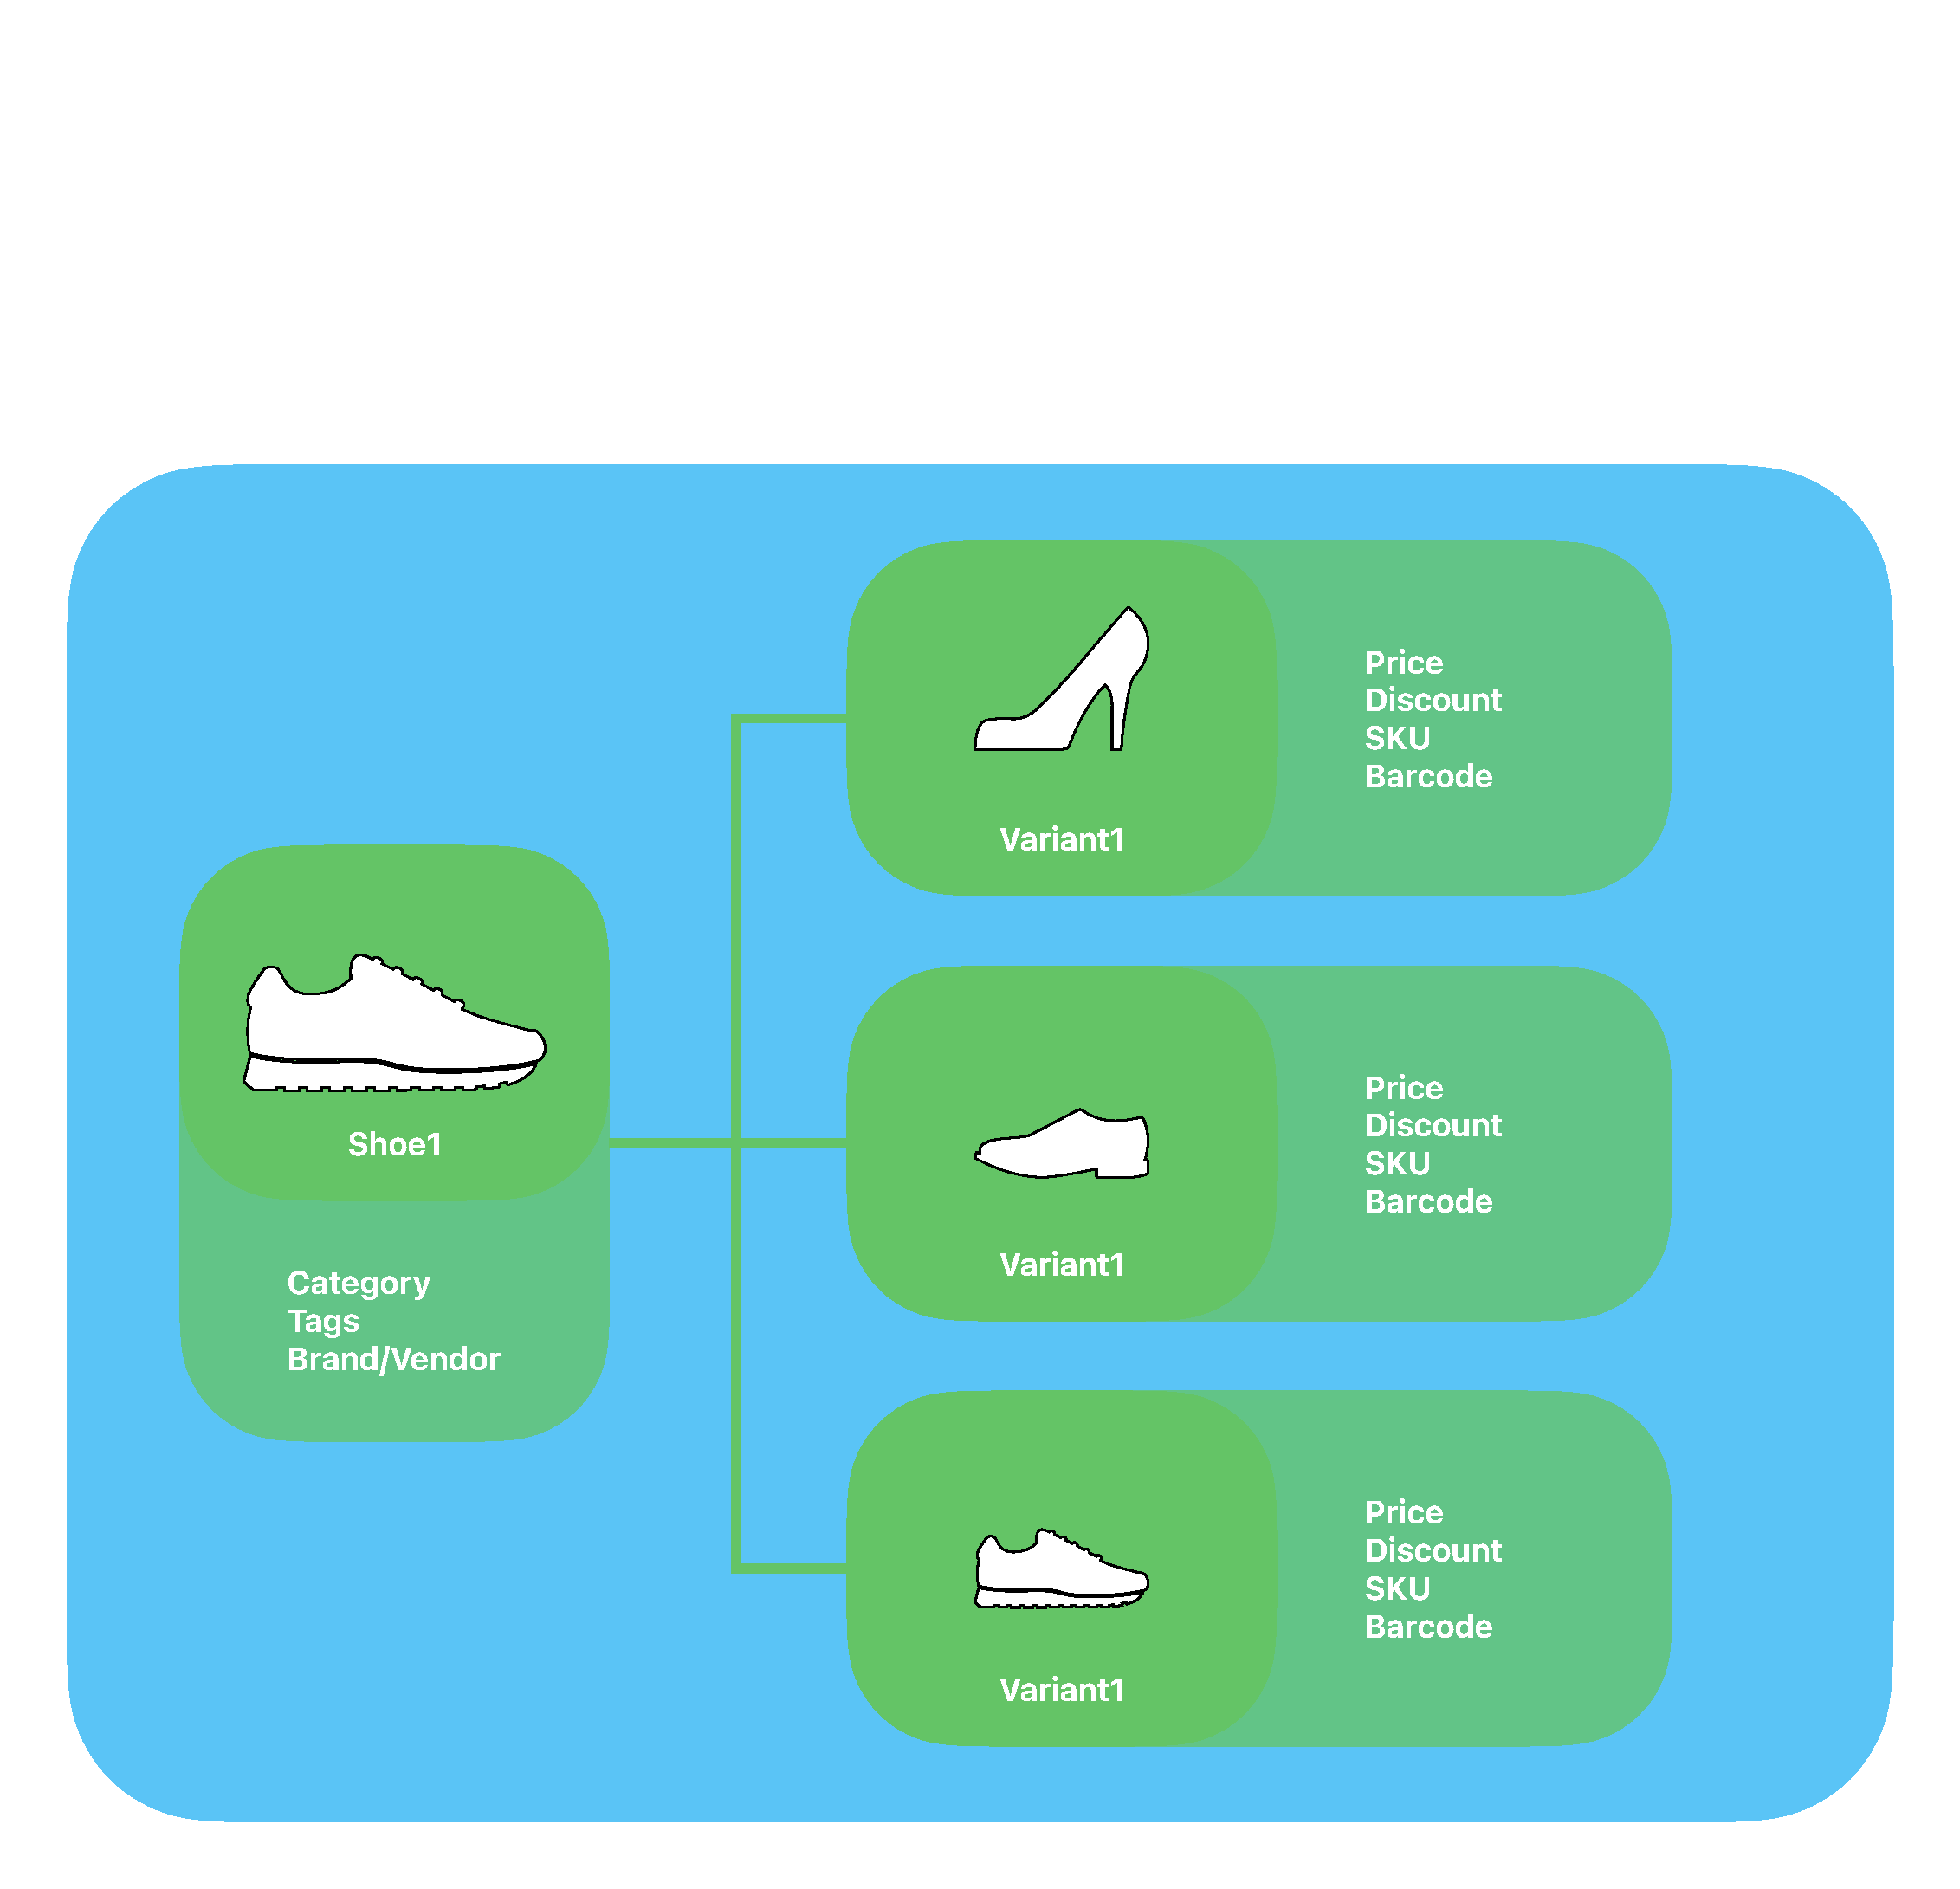
\includegraphics[width=\textwidth]{media/Product_variants.pdf}
    \caption{A product is comprised of different variants}
    \label{fig:rate_unlimited_comparison}
\end{figure}
Variants of the same product share some common product-level properties and each variant has its own differentiating variant-level properties. 


\section{The Need for Synchronization}
\begin{figure}[h!]
    \centering
    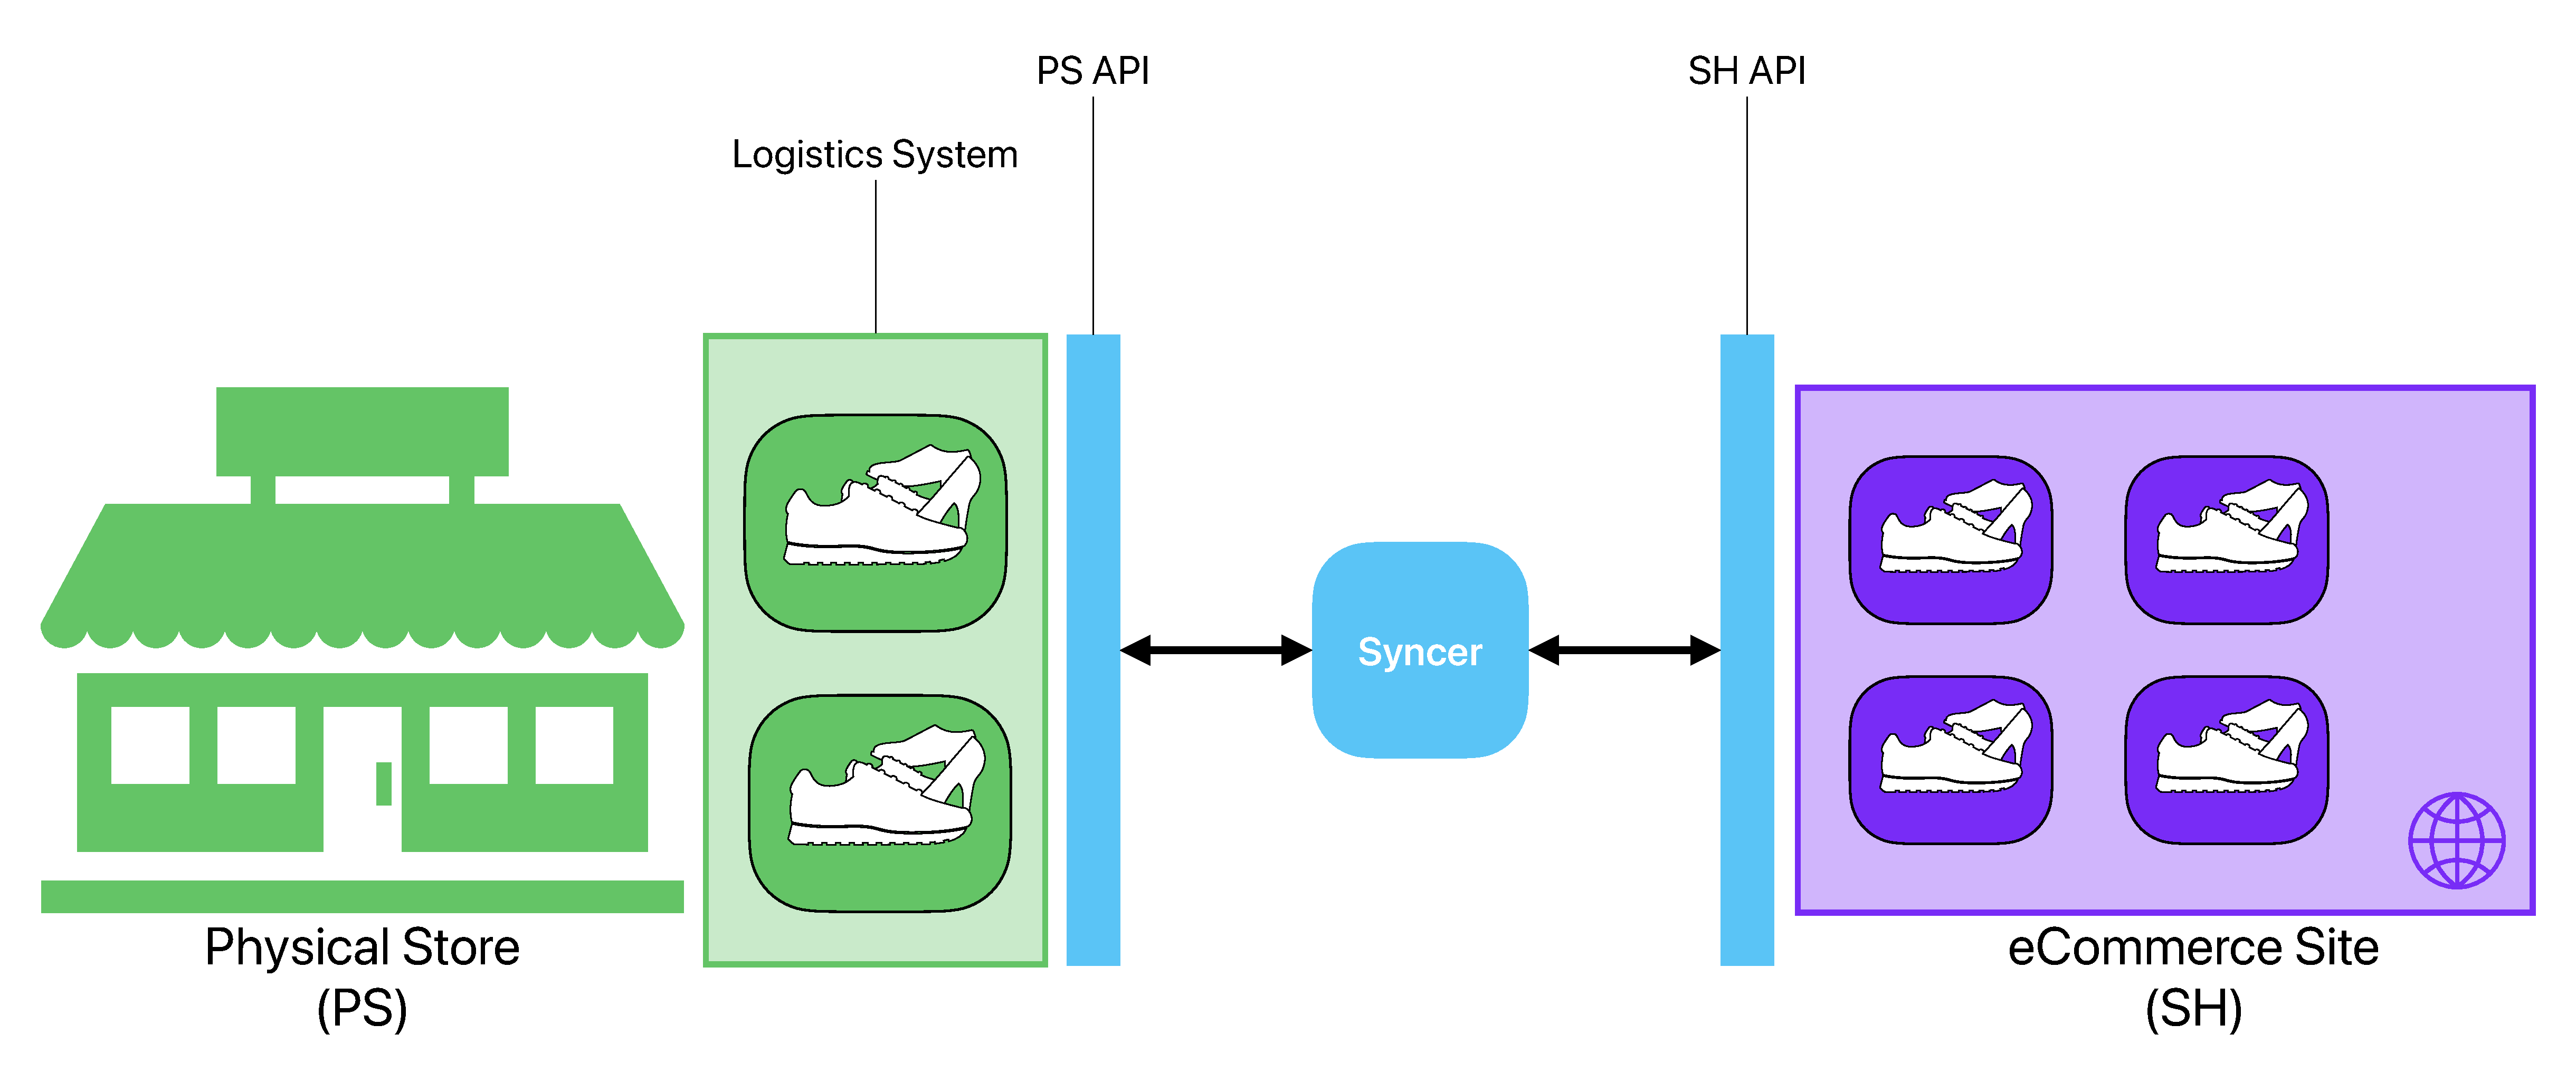
\includegraphics[width=\textwidth]{media/communications.pdf}
    \caption{High level outline of the problem scenario}
    \label{fig:case_comms}
\end{figure}
 Each product has different variants. The store keeps track of its inventory with a logistics system. That system provides an API endpoint with which one can query data and modify it.
The store wishes to have an online eCommerce store. The platform of the store has an API endpoint for adding and modifying resources, such as the products.
A system is needed that ensures that the online store reflects the current state of the physical store. That means that every product that exists on the physical store, should exist on the online store with the correct quantity. If a product sells out on the physical store, it is the job of the system to ensure that the lack of stock is present on the online store.
We will not focus on when the synchronization takes places but rather on how it would work.
\section{Sync Algorithm}
Since we're working with two separate systems, and most of our operations are network requests, there's a lot that could go wrong: a request could time-out, an endpoint might inexpectedly not accept a request or just be experiencing problems. Thus, we aim to minimize uncertainty.
Firstly, the current state of the product is retrieved. As shown in Figure 6.3, all relevant information about it is requested from each endpoint: the product, its variants and all its inventory listings.
\begin{figure}[h!]
    \centering
    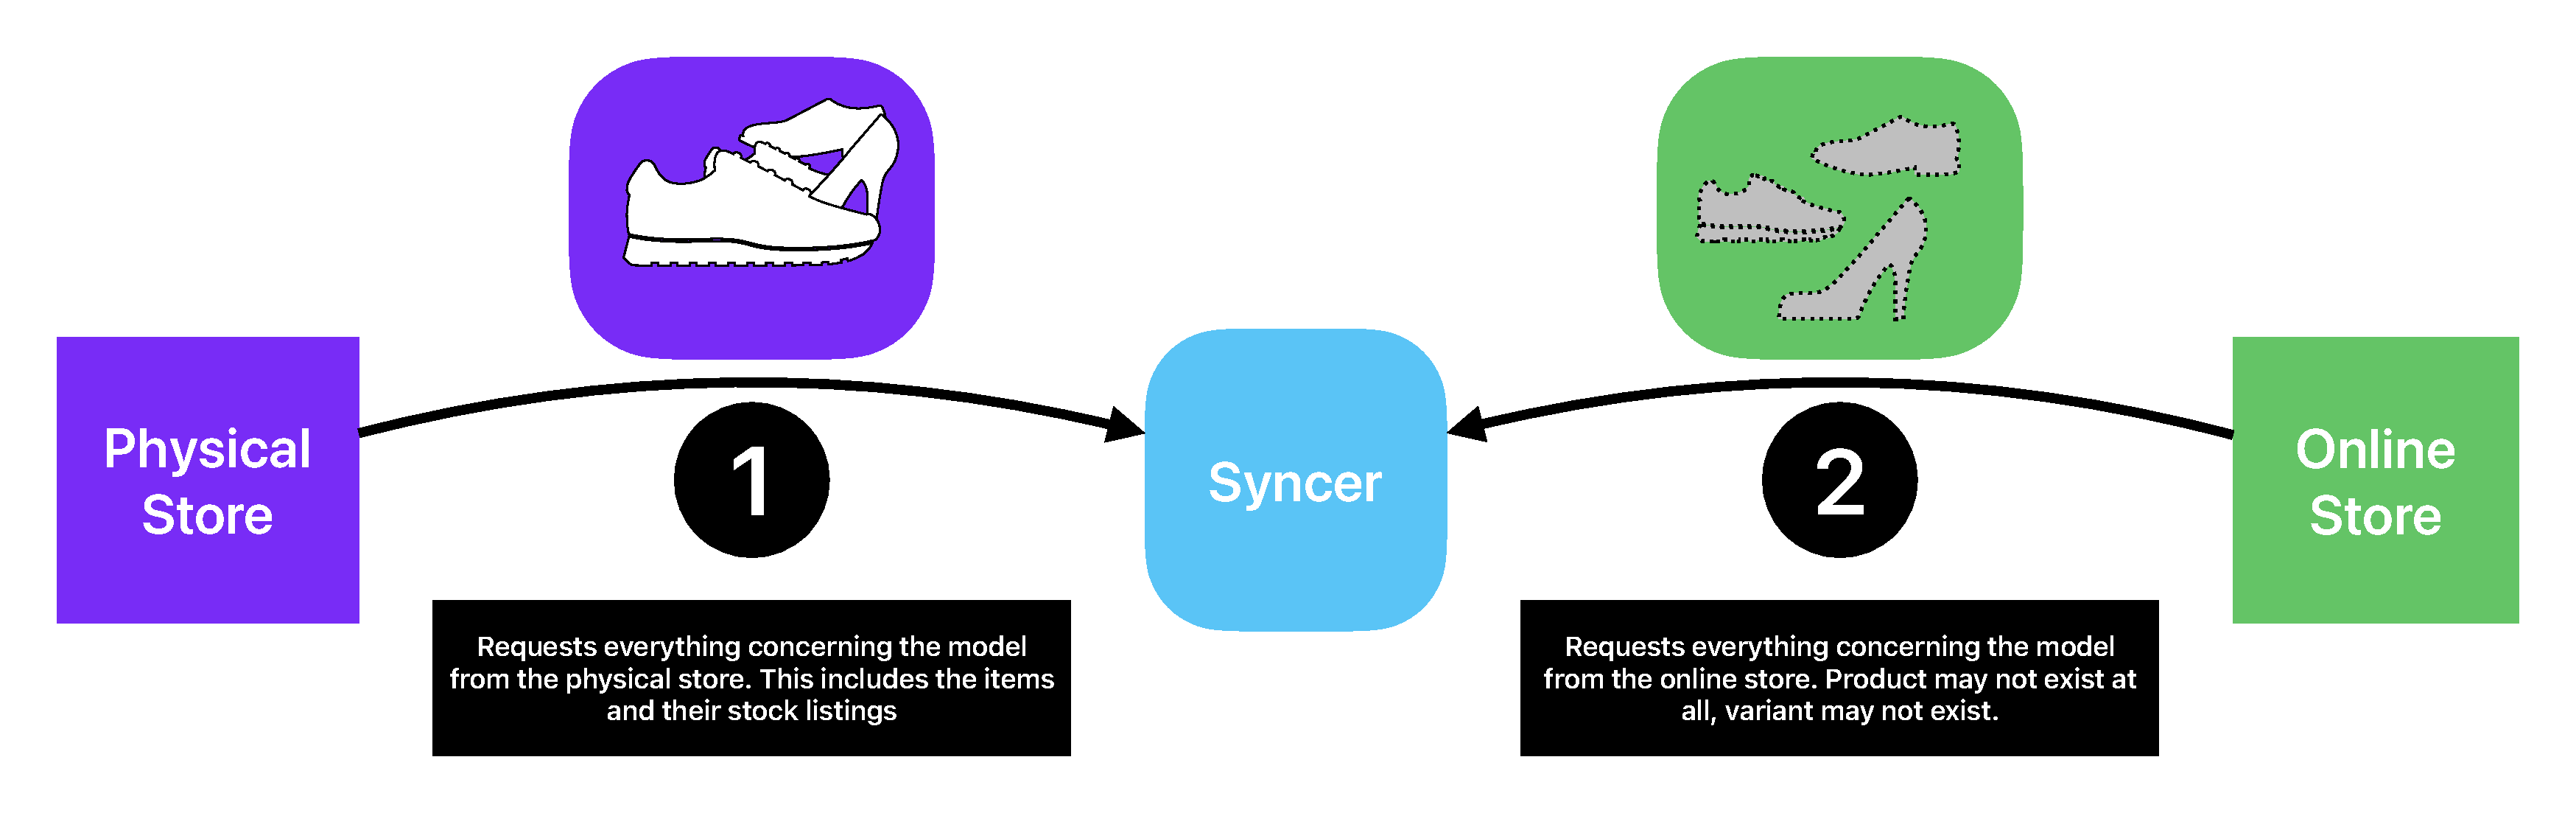
\includegraphics[width=\textwidth]{media/syncer_fetch_data_black.pdf}
    \caption{Steps 1-2: Fetching current data about the product}
    \label{fig:sync1_2}
\end{figure}
Continuing, we ensure the product-level properties are up to date. There is a case that an equivalent product on the online store might not even exist. It is at this step that the syncer constructs and creates it. Next step, as shown in Figure 6.4, is to do the same with the variant-level properties for each variant. The previous step ensures that an equivalent product does indeed exist. This is important, because at step 4 it means that we can safely assume only two cases for a variant: it exists or it doesn't. Finally, at step 5 we update each variant's inventory. Step 3 gaurantees that an equivalent product exists, and step 4 guarantees that an equivalent variant exists. This approach minimizes uncertainty. If any issues arise at any step, the sync is stopped, is marked as failed, along with the error that caused it.
\begin{figure}[h!]
    \centering
    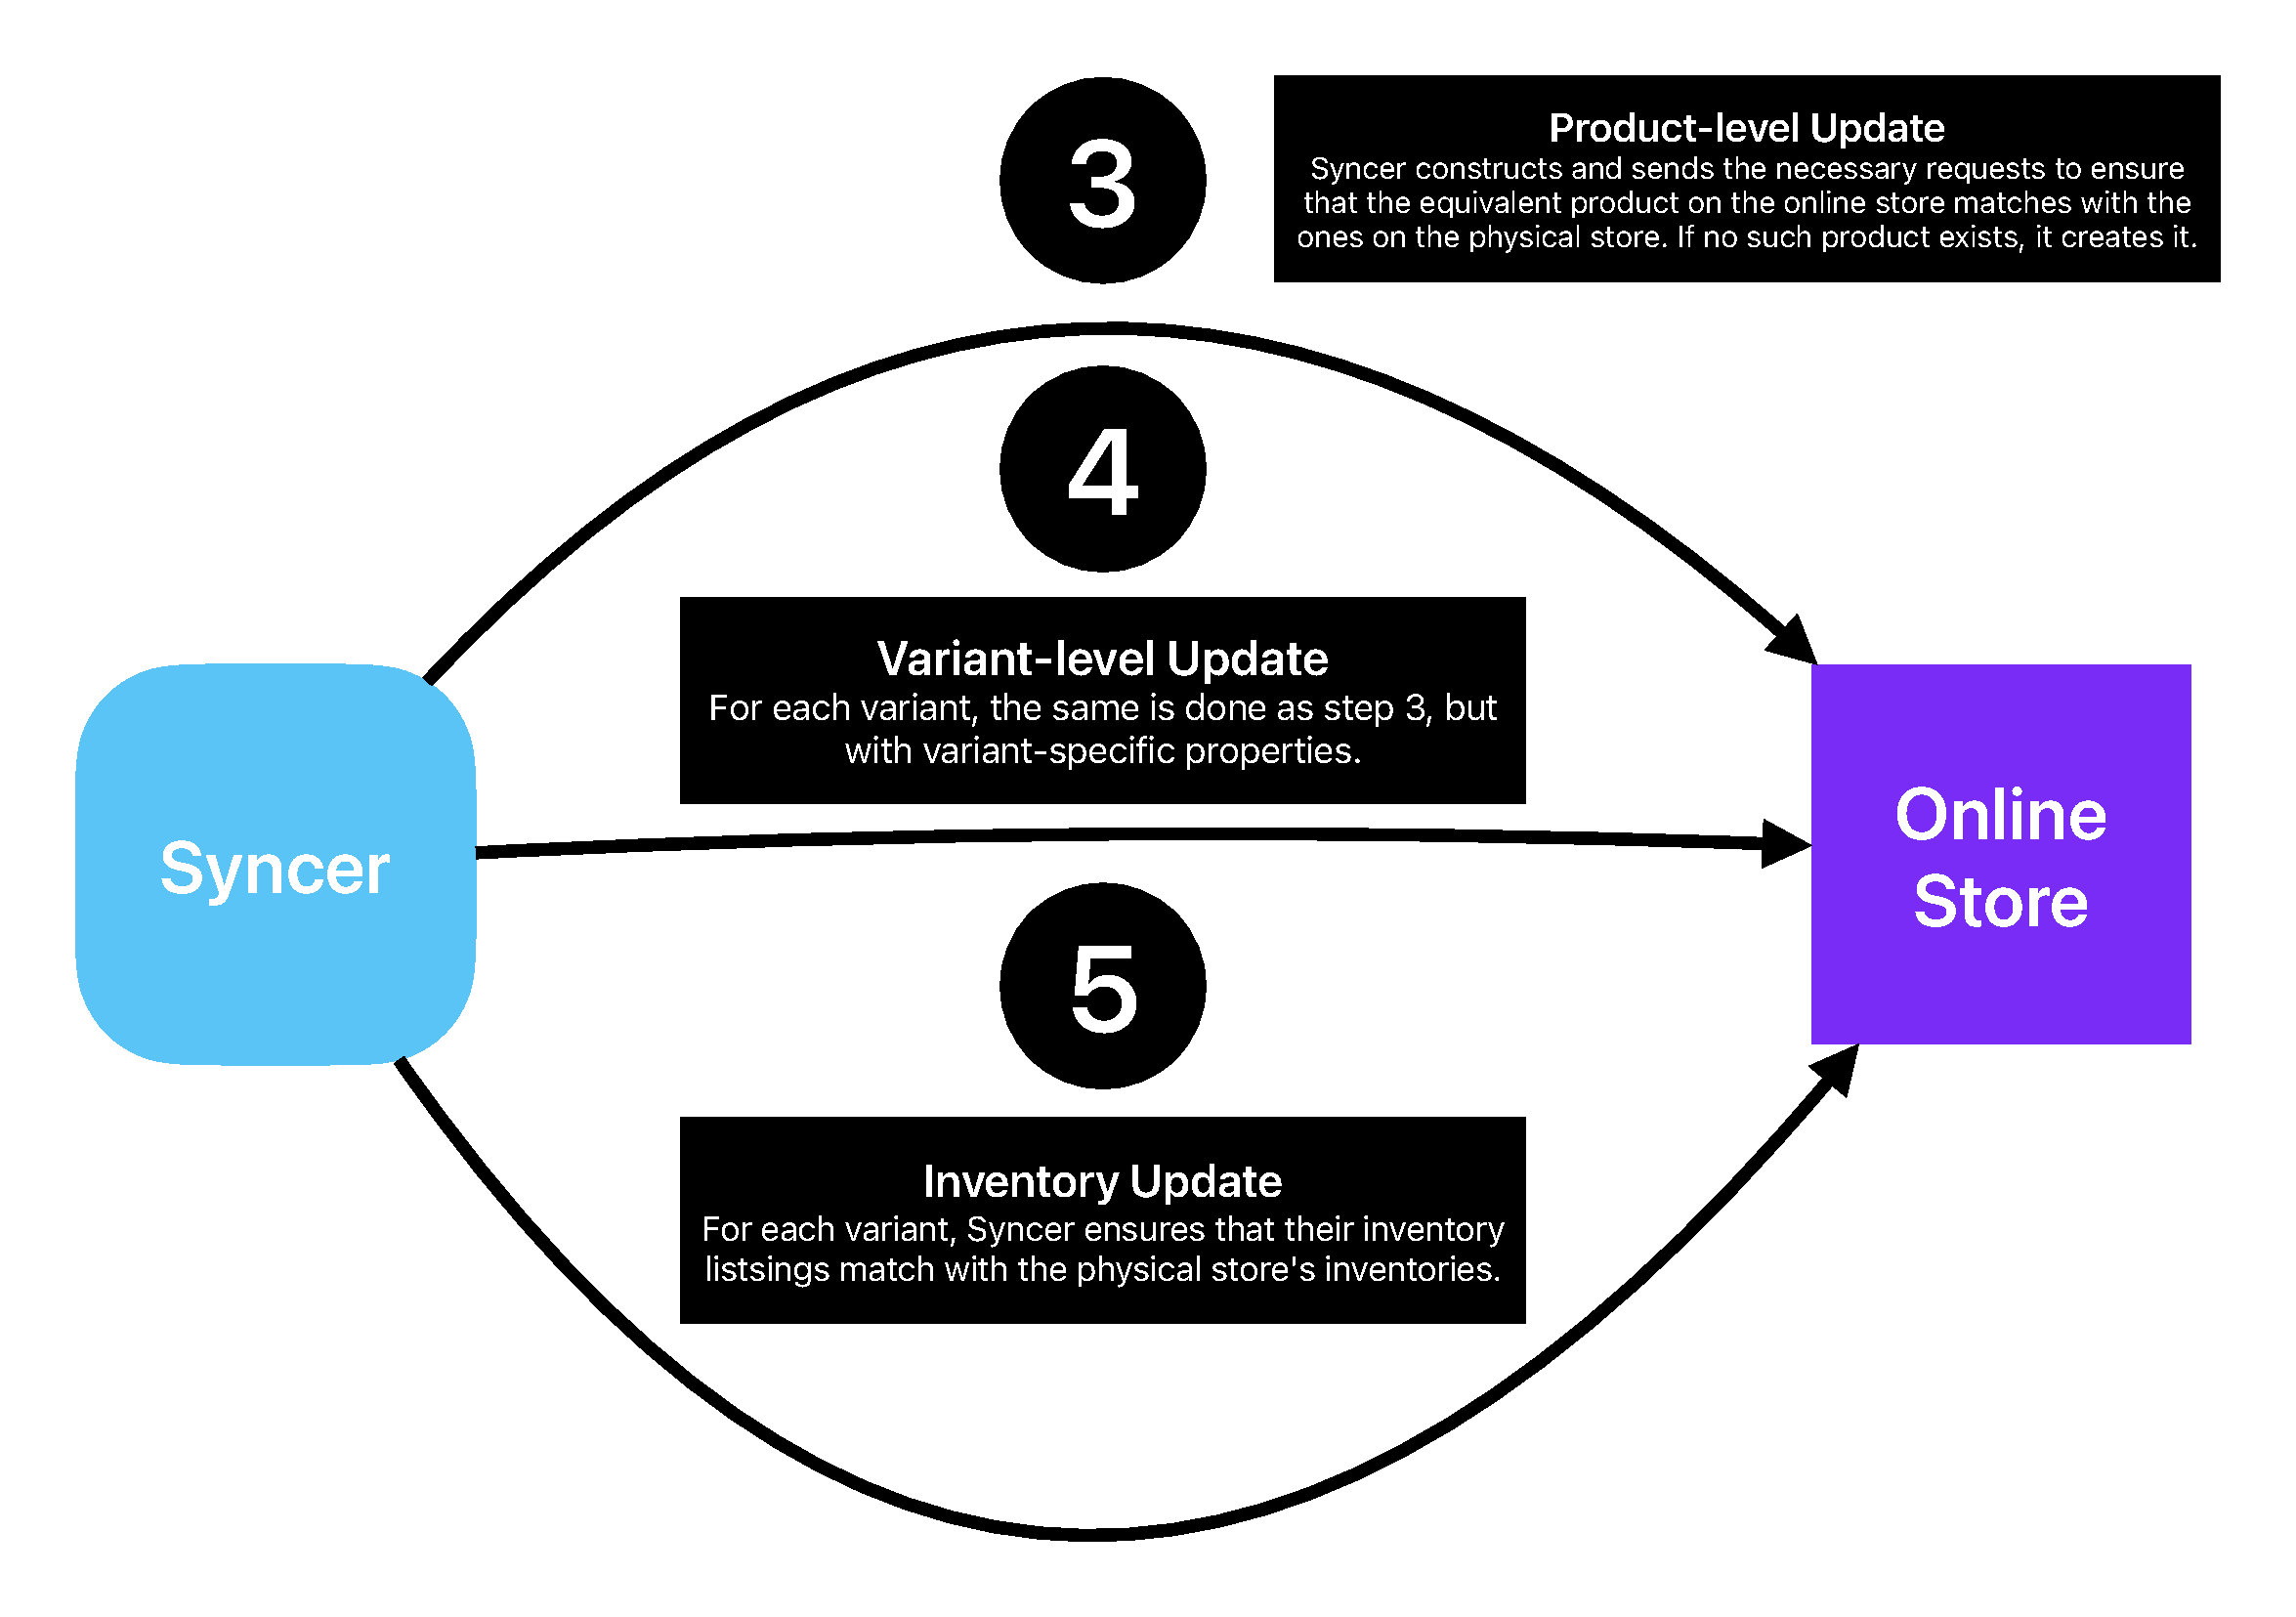
\includegraphics[width=\textwidth]{media/syncer_dosync_black.pdf}
    \caption{Steps 3-5: Apply any needed updates}
    \label{fig:sync3_5}
\end{figure}
\section{Implementation and Deployment}
Suppose we implement the above algorithm into a stateless function. It takes as input the model code (identifier of the product) and returns a descriptive type, that includes any possible errors and any modifications that it has done. We wish to use this function in a monolithic and serverless implmenetation, so we can later compare them. Since the function is stateless, we can easily define it as an action on OpenWhisk (Fig. 6.5). The input also contains the URLs of the PS and SH servers.
\begin{figure}[h!]
    \centering
    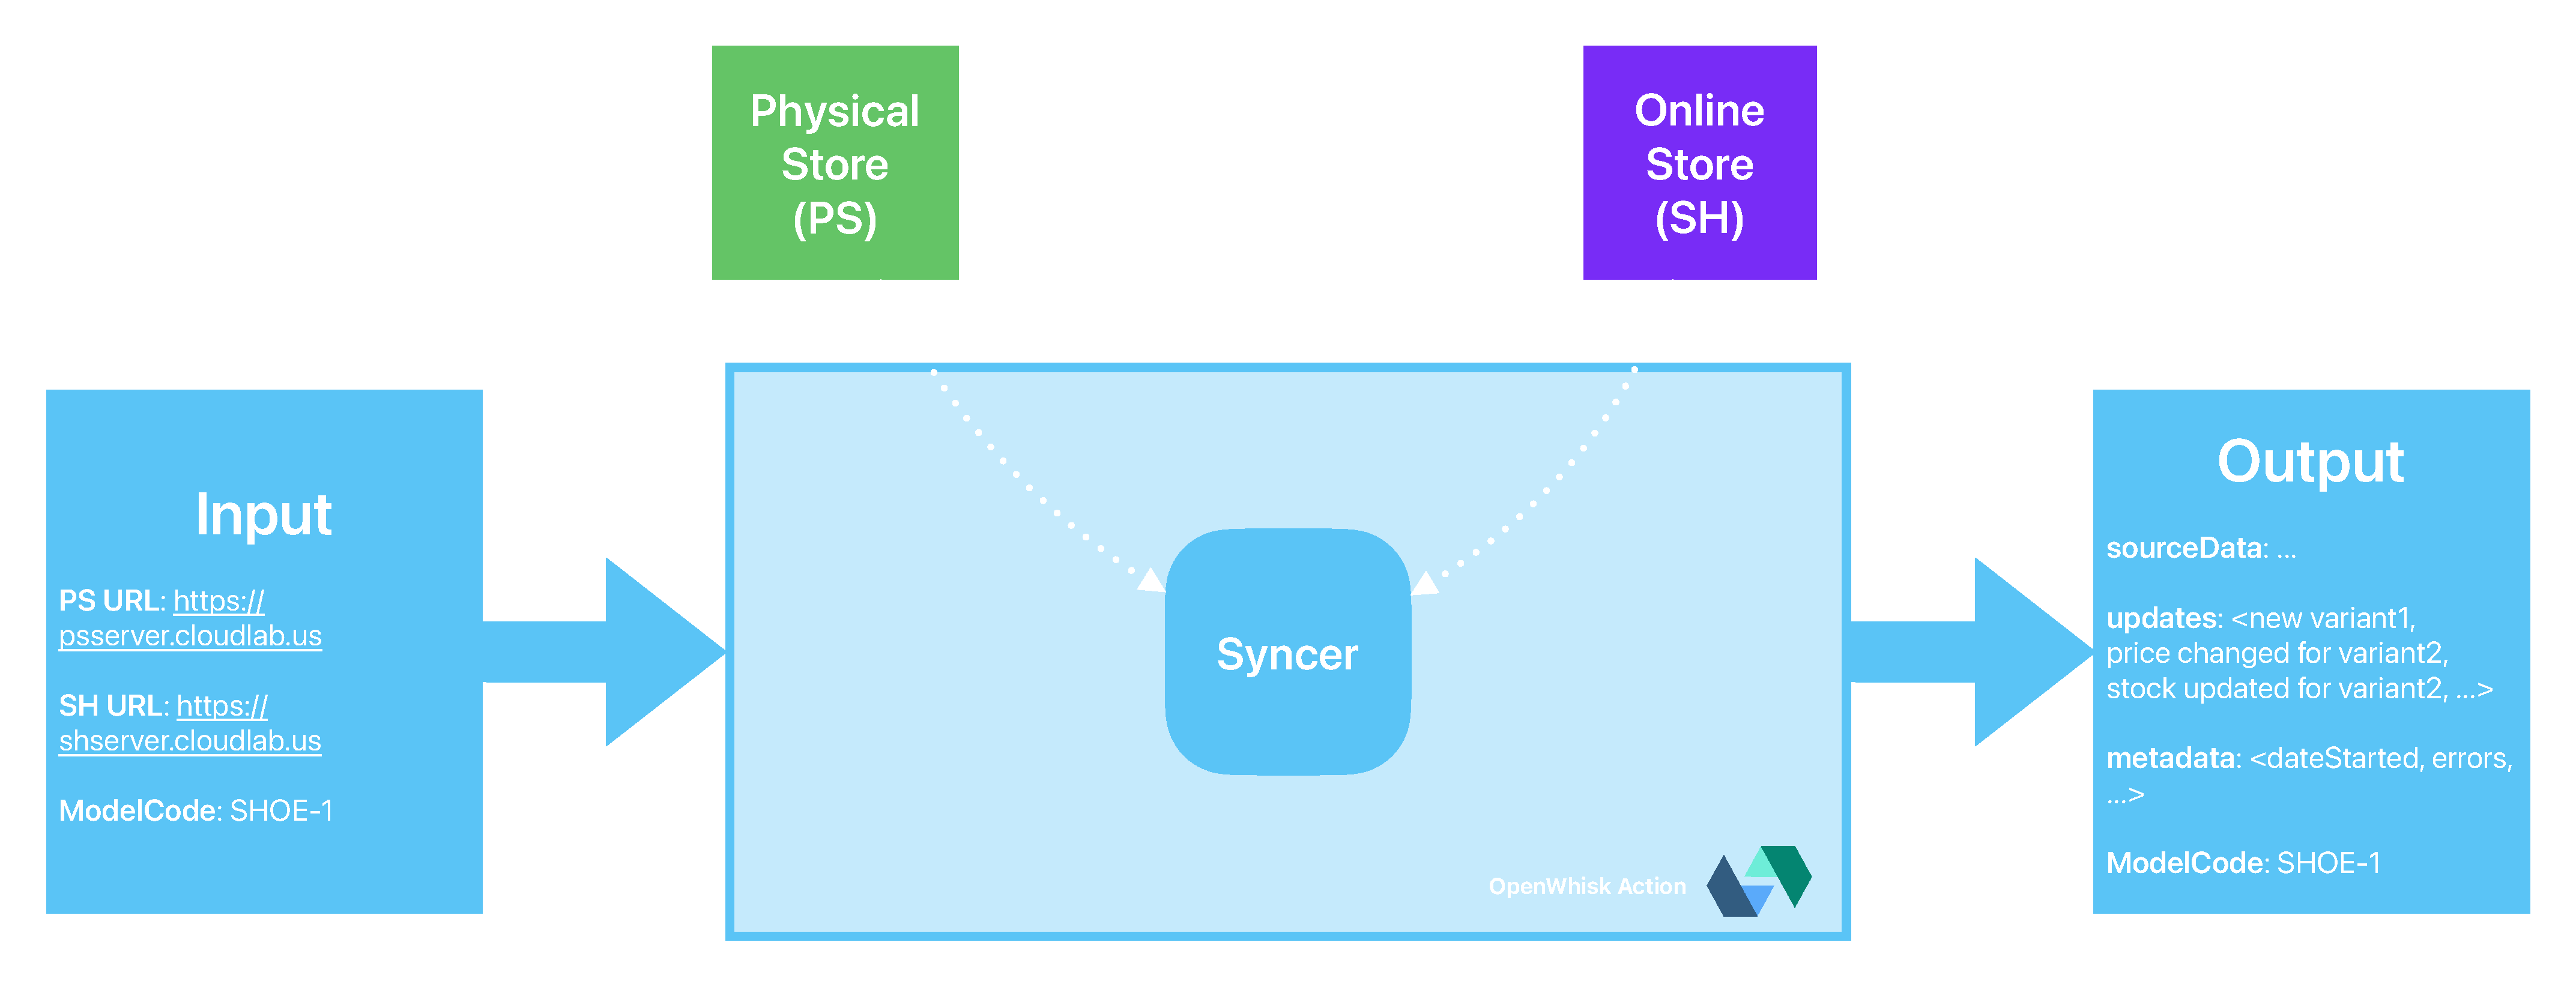
\includegraphics[width=\textwidth]{media/syncModelAction.pdf}
    \caption{Serverless Deployment}
    \label{fig:sync3_5}
\end{figure}
As for the monolithic implementation, we can set up a simple web server that exposes a route which accepts the same exact input as the OpenWhisk action, runs the same sync function, and returns its output (Fig. 6.6).
\begin{figure}[h!]
    \centering
    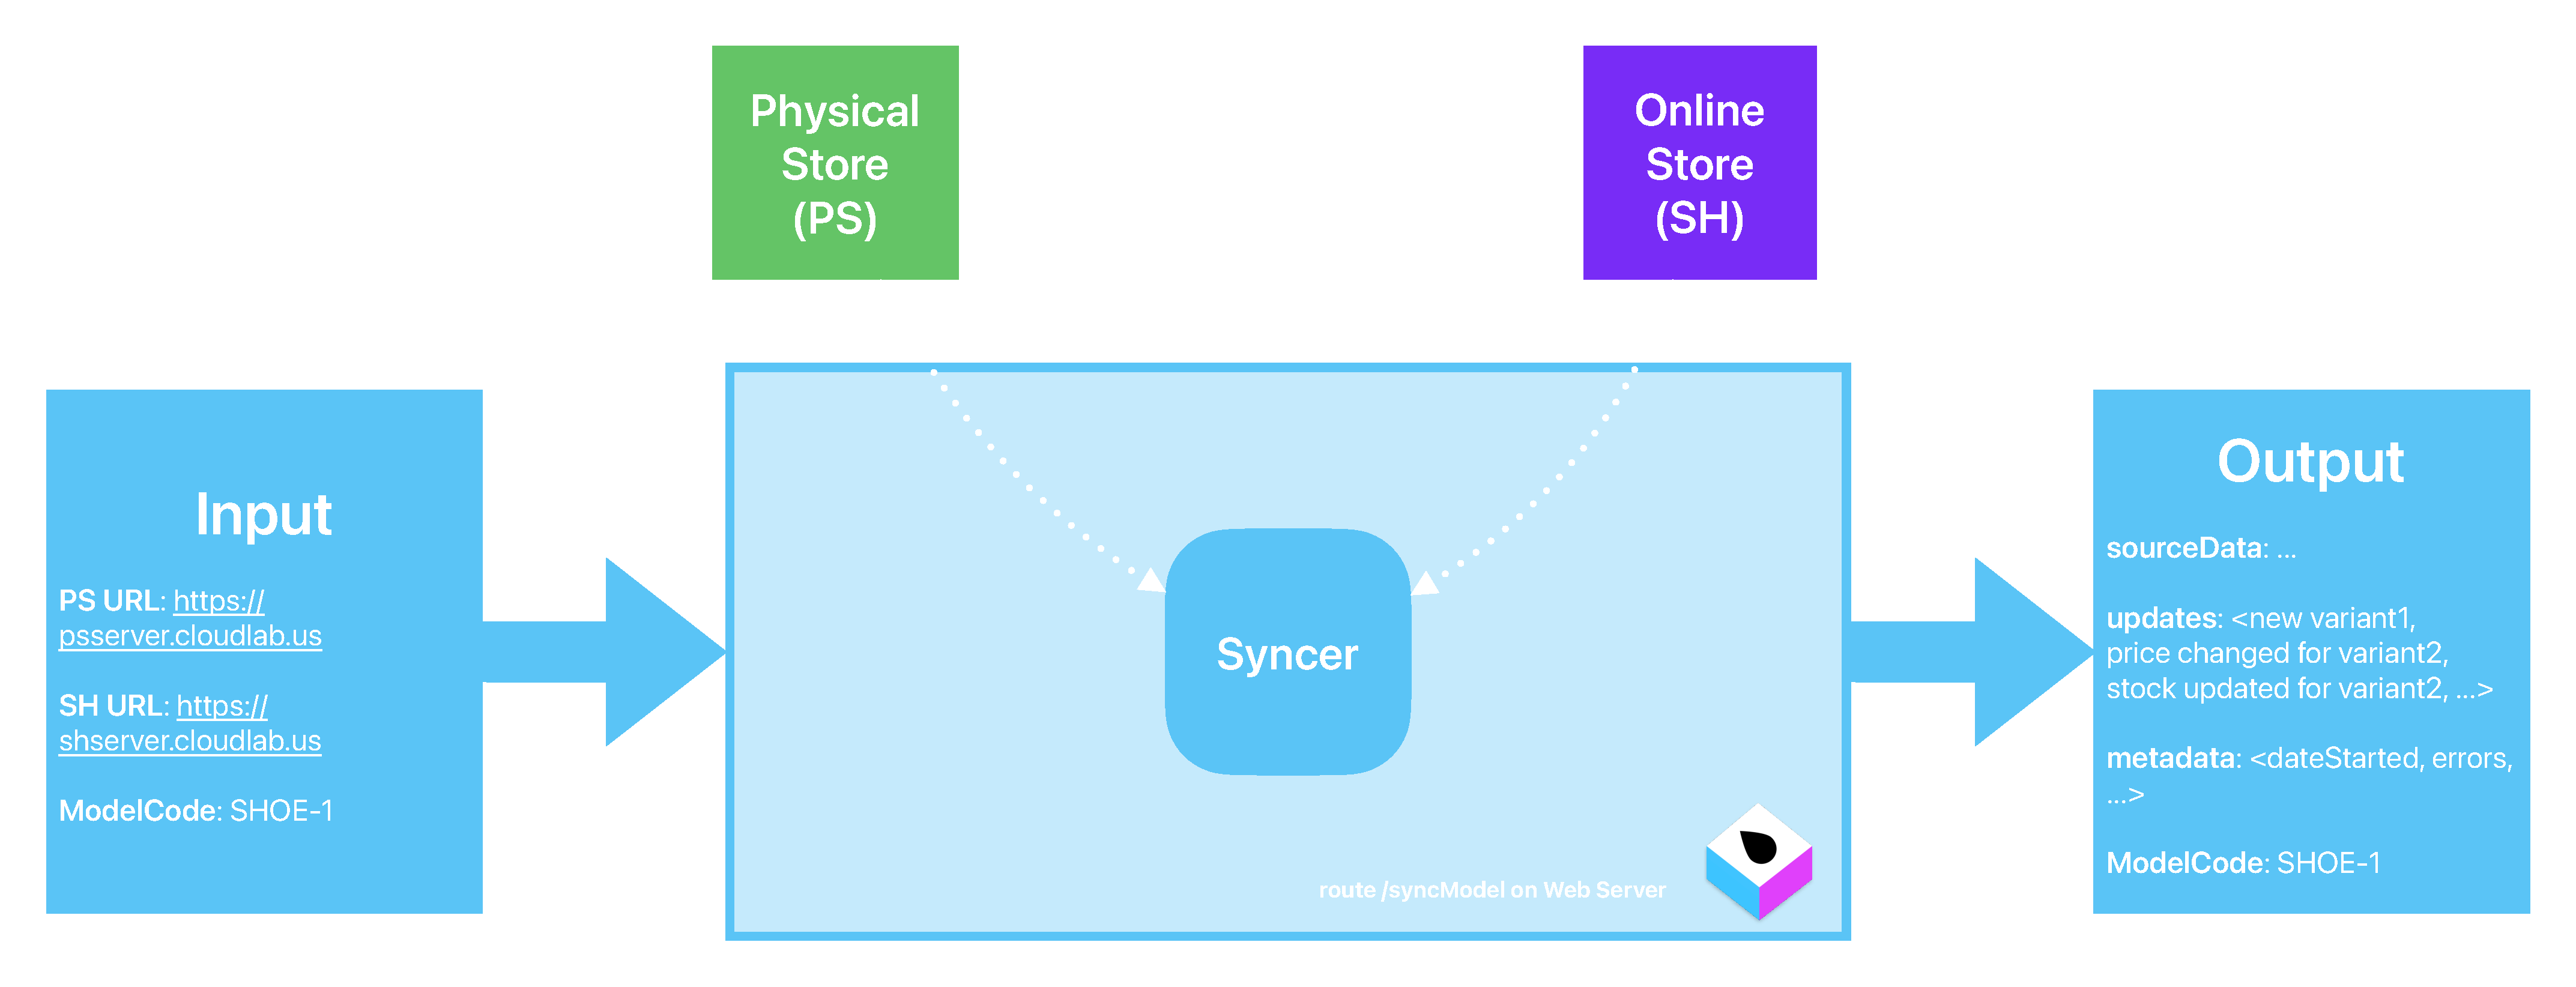
\includegraphics[width=\textwidth]{media/syncModelMonolithic.pdf}
    \caption{Monolithic Deployment}
    \label{fig:sync3_5}
\end{figure}


